\subsection{Time plot compared with fingerprints}
\label{section:TimePlotVsFingerprint}
The naive way to look at vibration signals is to use a time plot, which shows the amplitude over time. For anomaly detection though this is unsuitable due to overplotting \parencite[p.~2]{rakuschek2025visual} and lacks the ability to clearly represent the periodic behavior of a signal.

In time series data even a single snapshots contain a large number of individual data points. When plotted they merge into a continuous block that carries little information and adding more data to the plot only compresses this block further.

One of the main characteristics that can be exploited when working with vibration data is its
periodic behavior. Healthy baselines can be established, which then serve as a direct
comparison for data arriving later. A time plot, however, does not make this periodic
behavior visible. As shown in Figure~\ref{fig:BadExample}, blindly plotting a large number of
data points, in this case 20480 individual data points, results in a plot that carries little
information about the state of the machine.

\begin{figure}[H]
\centering
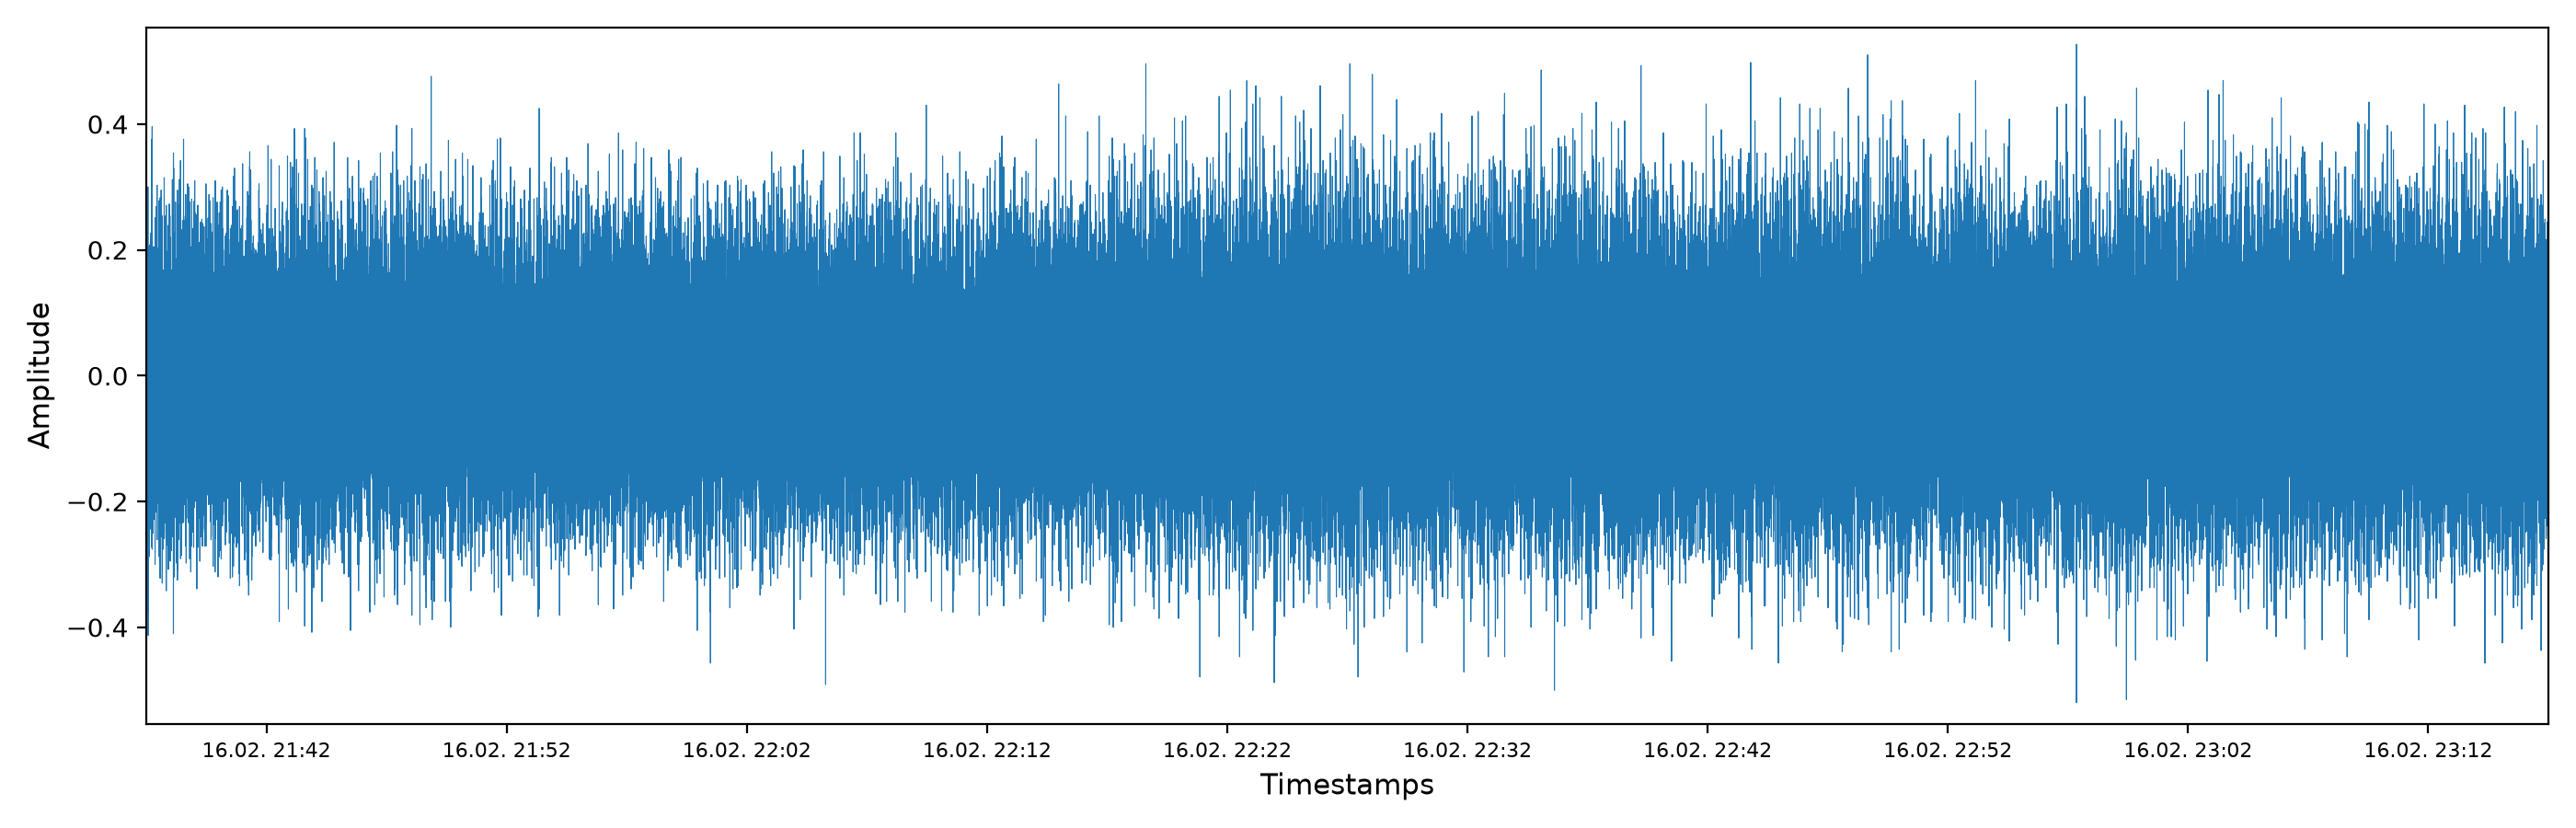
\includegraphics[width=1\textwidth]{figures/timePlotvsFingerprint/timeseries.png}
\caption{Example of the raw vibration signal.}
\label{fig:BadExample}
\end{figure}

\begin{figure}[H]
\centering
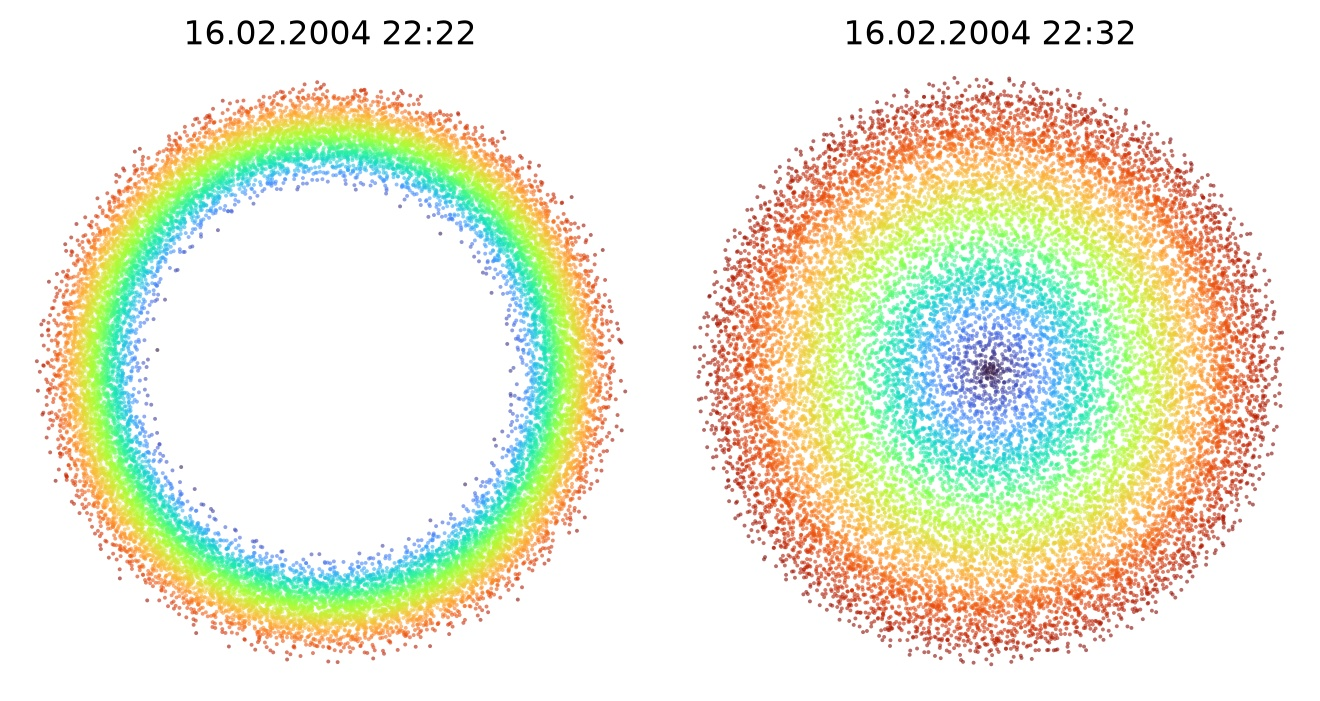
\includegraphics[width=1\textwidth]{figures/timePlotvsFingerprint/fingerPrintsVsTimeSeries.jpg}
\caption{Two fingerprints with clear visial distinction.}
\label{fig:healtyAndFaultyFingerprint}
\end{figure}


In contrast, transforming the data into a time delay embedding fingerprint results in a highly compact visually informative fingerprint.Figure \ref{fig:healtyAndFaultyFingerprint} shows two fingerprints taken at different times of the experiment. The left one shows the healthy state at the beginning the run as a clear continuous ring. The right plot, which was taken shortly before the failure occurred, shows a scattered point cloud with a filled center. Even without knowing anything about the method or the definition of healthy or faulty fingerprints the difference between the two representations is visible to the naked eye. If one leaves aside condition monitoring or fault forecast and just compares the time plot and the two fingerprint the time plot would not state with certainty that a fault even occurred. 

